\chapter{Analysis}\label{chap:analysis}

\section{Mapping}
Mapping \emph{actions} to joystick buttons and axes (\emph{controls} from now on) is the main feature of JSMapper. Its purpose is to be able to map actions such as pressing keys, moving mouse cursor, or even complex key sequences to the controls on any joystick and similar device. When the user operates the device, the specified action is played, and it's interpreted by the system just like if it were coming from a real hardware device.

Concepts related to the \emph{Mapping} feature are discussed below.

\subsection{Controls}
A device \emph{control} is any ``mechanic'' element on the input device (a joystick, a wheel drive, ...) to be operated by the user. JSMapper is currently able to map actions to the following controls on a device:
\begin{itemize}
	\item \emph{Buttons}: any kind of simple button, ``hat''-type buttons, mode switches, etc..., as long as they are reported as a \emph{button} by the device.
	\item \emph{Axes}: absolute axes such as X \& Y on a joystick stick, throttle, accel / break pedals, etc... Some devices also report ``hat''-type buttons as axes instead of buttons.
\end{itemize}

Any controls is defined as to be able to have always two possible states, ``active'' and inactive'', the exact meaning of which is different for every control type (see below). This abstraction, though, is used by the mapping engine so any action can be mapped to any control, no matter what their types are.

\subsubsection{Buttons}
As joystick buttons has only two possible states, pressed and released, theses are obviously mapped to activation states in a very straighforward way:
\begin{itemize}
	\item Pressed $\rightarrow$ Active
	\item Released $\rightarrow$ Inactive
\end{itemize}

This means that, when a button is pressed the assigned action will be ``active'' in its turn, and when the button is released the action will be inactive''. 

For the case of a simple \emph{Key} action, this means pressing down the mapped key when the button is pressed, and releasing it when the button is released.

\subsubsection{Axes}
Axis are more complex to map, as they don't provide two activation states but a large, continuous, range of values. For this reason, mapping actions to axes is made by defining \emph{Bands} on it, this is, intervals of values from within the whole range of the axis.

Actions are then mapped to individual \emph{Bands} on the axis, rather that on the whole axis itself. In conclusion, the ``activation'' state for the band is then defined by the current position of the axis at any time:
\begin{itemize}
	\item If inside the band $\rightarrow$ Active
	\item If outside the band $\rightarrow$ Inactive
\end{itemize}

This means that any number of different actions can be mapped to the same axis, as long as different, not overlapping bands are defined for it. Figure \ref{fig:axis_mapping} shows an example of how four actions can be mapped to an axis by assigning them to different bands across the whole axis range, while keeping an ``inactive'' section at the center (acting as a ``dead'' zone, i.e.).

\begin{figure}[htb]
\centering
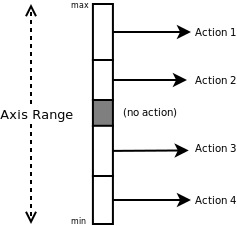
\includegraphics[width=0.5\textwidth]{axis_mapping}
\caption{Axis mapping through bands}
\label{fig:axis_mapping}
\end{figure}

The same idea is applied in order to use \emph{axis bands} as activation conditions for \emph{Modes}.


\subsection{Actions}
An \emph{Action} represents the event to ``simulated'' or (``played'') whenever the source control the action is mapped to is operated. 

To match \emph{controls} design, actions also have two possible states, ``active'' and ``inactive'', the exact meaning of which depends on the action type. The mapping engine will thus ``activate'' an action when its source control gets ``active'', and ``deactivate'' it when control gets back to ``inactive'' status.

Currently, JSMapper supports 3 types of actions:
\begin{itemize}
	\item Key actions
	\item Axis actions
	\item Macros actions
\end{itemize}

All action types share a common attribute, named \emph{filter}: if this attribute is set to true, then the original event sent by the hardware input device driver is filtered out, so it's not receuved by the system. If false, then event wil keep its way upstream to the chain of event handlers after executing the associated action.


\subsubsection{Key actions}
This is the most simple action, designed to simulate key press \& release events (``keystrokes''). This action type is suitable to be used for simulating the entry of either single keys, or either shortcut-alike keystrokes, as it supports an optional ``modifiers'' mask for this sake.

Mouse button actions are also simulated through this action: in such a case, instead of a key identifier a mouse button identifier is used.

These are the attributes of a \emph{Key} action:
\begin{itemize}
	\item \emph{key}: Linux kernel code of the key (or mouse button) to simulate.
	\item \emph{modifiers}: a mask indicating an optional use of \emph{Shift}, \emph{Control}, \emph{Alt} modifiers keys.
	\item \emph{single} flag: a flag indicating if the key will self-repeat or not
\end{itemize}

Key actions behaves differently depending on the value of the \emph{single} flag:
\begin{itemize}
	\item If true, then the key will be ``pressed'' and immediately released whenever source control gets activated, thus only a single key (or shortcut) will be issued. No action will be taken on source control deactivation.
	\item If false, then the key (and the modifiers) is ``pressed'' when the source control gets ``activated'', and ``released'' when the source control gets ``inactive''. As the simulated key will remain ``pressed'' until then, the system will self-repeat the key for as long as it's hold down, just like if a real key on the keyboard is pressed and held down.
\end{itemize}


\subsubsection{Axis actions}
Axis actions are designed to simulate movement in any of the \emph{relative} axes supported by Linux input subsystem, particularly the X \& Y axes used by mouse devices. This way, it's possible to use the joystick to move the mouse on screen.

These are the attributes of an \emph{Axis} action:
\begin{itemize}
	\item \emph{axis}: Linux kernel code of the axis to simulate movement for.
	\item \emph{step}: an integer values indicating the number of axis units to perform per step
	\item \emph{single} flag: a flag indicating a single-step movement or a continuous one.
	\item \emph{spacing}: in continuous mode, the spacing (in ms) between steps
\end{itemize}

In a similar way to \emph{Key} actions, \emph{axis} also behave differently depending on the value of ``single'' flag:
\begin{itemize}
	\item If true, a single movement will be made, of the magnitude indicated by the ``step'' value. The movement will be peformed at source control ``activation''.
	\item If false, then the action will generate a continuous movement on the axis, for as long as the source control is kept ``activated''.
\end{itemize}


\subsubsection{Macro actions}
Macro actions permits automating a number of basic keystroke events which will get executed in a row, thus the name of ``macro'' assigned to them. Every keystroke of the macro can be defined either as a single key, or either include an optional ``modifiers'' mask, just like \emph{Key} action.

These are the attributes of a \emph{Macro} action:
\begin{itemize}
	\item \emph{keys}: an array of keystroke definitions, this is, a key code and an optional ``modifiers'' mask.
	\item \emph{spacing}: the spacing left between keystrokes (in ms).
\end{itemize}


Behaviour of \emph{Macro} actions is always the same: the entire sequence of keys is launched whenever the source control gets ``activated'', without any possibility to cancel it. No action is done on source control deactivation.


\subsection{Modes}
Modes are an integral part of JSMapper, and one of its most advanced features. Put short, modes are different sets of mapping assignments that coexists at the same time, and which are selectable at runtime by the user by operating i.e. a switch or a button on the joystick.

Modes are organized hierarchically, so there is always a \emph{root} mode, which contains the common assignments (or any at all...), then any a number of optional child submodes (which, in its turn, can contain more submodes by themselves).

\subsubsection{Conditions}
Children submodes must feature an \emph{activation condition}, which is the condition that must be met in order for the mode to be \emph{active}: this condition can be either a button being pressed, or else an axis fitting a determined range of values (a \emph{``band''}).

Two types of activation condition are supported:
\begin{itemize}
	\item \emph{By button}: if the button is pressed, the mode is active, else is inactive.
	\item \emph{By axis band}: if axis current value is inside the band, the mode is active, else is inactive.
\end{itemize}

\subsubsection{Mode switching}
At runtime, the mode to be applied for every button (or axis) at a given time is determined in the following way:
\begin{itemize}
 \item First, starting with root mode, the driver checks if the activating condition of any of its children modes is met. If so, then it repeats the process by starting from that mode, and then recursively, until it can't go further down the mode hierarchy.
 \item Then, starting from the last mode found, it checks if it contains an assignment for the button and, if so, the associated action is launched. Else, the driver goes up one level and repeats the check with the parent mode, until eventually it gets back to \emph{root} mode if no action is found in any submode.
\end{itemize} 


The way mode selection works, it means that a given child mode can be active \emph{only} if its parent mode is: this is, it's OK to use the samer activation condition for two children modes, as long their respective parent (which must not be the same) have different activation conditions on their own:

\begin{figure}[htb]
\centering
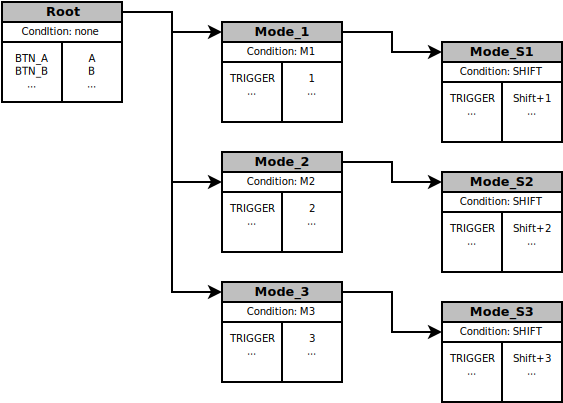
\includegraphics[width=1.0\textwidth]{modes}
\caption{Modes in cascade}
\label{fig:modes}
\end{figure}

Figure \ref{fig:modes} displays an example of a profile for the Saitek X-45 containing the mandatory \emph{root} mode mapping some basic buttons, plus 3 submodes which get selected by a 3-position switch on the joystick (which internally gets translated to 3 different buttons, labeled ``M1'', ``M2'' and ``M3''). In its turn, each one of these submodes contain another child submode, which is activated by the ``SHIFT'' button.

With this setup, the profile will behave in the following way:
\begin{itemize}
	\item For ``A'' or ``B'' buttons, the driver will always emit the corresponding action mapped by \emph{root} mode, as it's not overriden by any of the submodes.
	\item For ``TRIGGER'' button, the driver will initially choose the appropiate submode by checking the state of the ``M1'', ``M2'' and ``M3'' buttons. Then, it will check ``SHIFT'' in order to decide if the \emph{shifted} child mode must be used: if so, then the action from the shifted submode will be emitted, else the one from the submode.
\end{itemize}


\section{Driver API}
As seen on previous chapters, the \emph{jsmapperdev} kernel module creates a \emph{jsmapXX} device node under \emph{/dev/input/} for every gaming-type device attached to the sysrem. These device nodes are the entry point for the userspace API, which is used to load profiles into the driver, this is, mapping actions to device controls.

A program wanting to interact with the device would open the device node (using regular \emph{open()} system calls), then issue the required \emph{ioctl()} calls to load the whole mapping set into the driver.

These are some of the IOCTL control code supported by the API:
\begin{itemize}
 \item \textbf{JMIOCGVERSION}: returns API version
 \item \textbf{JMIOCGNAME}: returns associated device name
 \item \textbf{JMIOCGBUTTONS}, \textbf{JMIOCGAXES}: returns number of buttons / axes in device
 \item \textbf{JMIOCCLEAR}: clears device mapping
 \item \textbf{JMIOCSBUTTONACTION}: assigns an action to the given button
 \item \textbf{JMIOCSAXISACTION}: assigns an action to a band of the given axis
 \item \textbf{JMIOCADDMODE}: adds a new mode
\end{itemize}

The whole set of IOCTL codes supported by the API, along with the structures to be passed as parameters, are defined in the \emph{jsmapper\_api.h} header file.


\section{Profiles}
Mapping profiles are XML files containing the definition of the mapping to be to load into the device. They can be create using a regular text editor, and contains the whole list of actions, modes, mappings, etc... that can be atomically loaded into the device.

The user is expected to create a profile for every game it/she want to play with the device, every profile contaning the mapping from device controls to game actions, by means of simulated keyboard and mouse actions.

Check annex \ref{chap:usermanual} ``User manual'' for complete profile format documentation.


\subsection{Device Maps}
\emph{Device maps} are special XML files that provide mapping between joystick elements ``natural· names and their related kernel numerical ID. They are needed because there is no easy way to obtain the ''actual`` name of an element, other than for the very basic X \& Y axes and some specific buttons (''FIRE``, i.e.).

Device maps thus, provide a way to make writing a profile an easier task by providing easy-to-remember names for the elements, so instead of referring to them by a raw number a more ''natural'' name can be used.

A bunch of device map files are shipped with the project, and JSMapper userspace tools will automatically try to use them, by finding the appropiate one on a device name basis. 

An special CLI tool (\emph{jsmapper-device}) is included to make writing \emph{device map} files an easier task. 


\subsection{Profile loading}
Profiles can be loaded into the device by using the provided \emph{jsmapper-ctrl} tool, which is the userspace CLI-based tool for JSMapper. 

Example~\ref{lst:jsmapper_ctrl_load} shows how to load a profile into the device:
\begin{lstlisting}[language=bash,caption={Loading a profile},label={lst:jsmapper_ctrl_load}]
$ jsmapper-ctrl -l profile.xml 
\end{lstlisting}

The same tool can be used also to clear the state of the driver, so it stops filtering and restores normal device behaviour, as displayed in example~\ref{lst:jsmapper_ctrl_clear}:
\begin{lstlisting}[language=bash,caption={Clearing device},label={lst:jsmapper_ctrl_clear}]
$ jsmapper-ctrl -c 
\end{lstlisting}

